\documentclass[12pt, letterpaper]{article}
\usepackage[utf8]{inputenc}
\usepackage{amsmath}
\usepackage{amsthm}
\usepackage{amssymb}
\usepackage{colortbl}
\usepackage[a4paper, total={6.5in, 10in}]{geometry}

\usepackage{graphicx}
\graphicspath{ {/} }
\newtheorem{problem}{Problema}
\title{Computación Concurrente - Tarea 2}
\author{Damián Rivera González\\Alexis Hernandez Castro}

\begin{document}
\maketitle


\begin{itemize}
\item[1. ] 1.Considera el algoritmo de Peterson:\\

\begin{center}
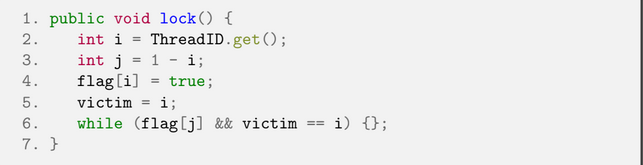
\includegraphics[width=0.7\textwidth]{pettersonCode.png}\\
\end{center}
\begin{itemize}

\item[a) ] Sup\'on que intercambias las l\'ineas 4 y 5. ¿El algoritmo sigue cumpliendo
con las propiedades de exclusi\'on y no deadlock? Demuestra o da una
ejecuci\'on en donde no se cumpla.

\item[b) ]Sup\'on ahora que la instrucci\'on de la l\'inea 6 se cambia por:
\begin{center}
$while(flag[j]$ \&\& $victim == j)$
\end{center}
Da un ejemplo en donde se cumpla la exclusi\'on mutua y otro en donde no.

\end{itemize}


\item[2. ]Considera el siguiente algoritmo para dos procesos:

\begin{center}
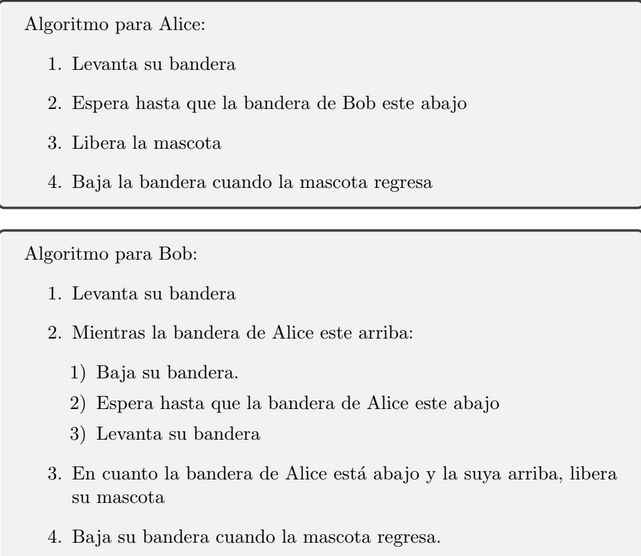
\includegraphics[width=0.7\textwidth]{aliceCode.png}\\
\end{center}



\begin{itemize}

\item[a) ]Demuestra que resuelve el problema de la exclusi\'on mutua.
\item[b) ]Demuestra por qu\'e no cumple con la propiedad libre de hambruna.
\item[c) ]El algoritmo cumple con la propiedad de no deadlock?
\item[d) ]Cu\'al es la desventaja del algoritmo? Argumenta por qu\'e es dif\'icil de
generalizar.
\end{itemize}


\item[3. ]Sup\'on que tienes la instrucci\'on swap(A,B) que intercambia de manera at\'omica los valores de las variables A,B.

\begin{itemize}
\item[a) ]Da una propuesta de codificaci\'on para un objeto Look que resuelva el problema de la exclusi\'on mutua para dos procesos.
\item[b) ]Demuestra que tu algoritmo cumple con la propiedad de exclusi\'on y no deadlock.
\end{itemize}

\item[4. ] Considera la siguiente modificaci\'on de la clase contador, que es ejecutada por dos procesos concurrentemente cuyos ID\' s son (0 y 1):


\begin{center}
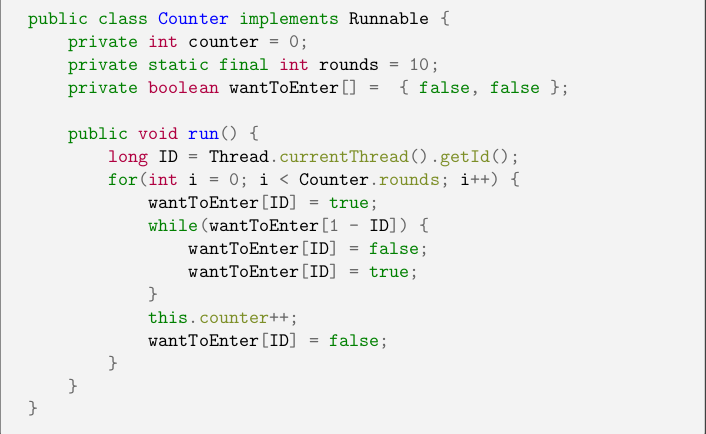
\includegraphics[width=0.7\textwidth]{CounterCode.png}\\
\end{center}


\begin{itemize}
\item[a) ]Muestra una ejecuci\'on en donde los hilos llegan a un estado de deadlock. 

\item[b) ] Demuestra que el algoritmo no tiene una condici\'on de carrera, es decir, toda ejecucin que termina siempre imprime el mismo resultado.
\end{itemize}



\item[5. ]¿Porqu\'e requerimos definir una secci\'on de entrada (doorway), porqu\'e no podemos definir un algoritmo de exclusi\'on mutua que cumpla con la propiedad FCFS basado en el orden en el que los hilos ejecutan la primer instrucción del m\'etodo lock? Argumenta tu respuesta caso por caso seg\'un la naturaleza de la primera instrucción ejecutada por el método lock(): una lectura o una
escritura, a registros separados o a un mismo registro.\\
Respuesta:\\

Cualquier algoritmo de exclusi\'on mutua consiste en c\'omputo y espera. Al dividir el c\'odigo en una secci\'on de puerta seguida de una sección de espera, movemos todo el c\'alculo al frente (en lugar de intercalar el c\'alculo y la espera). Esto impone una estructura limpia al algoritmo y facilita el reconocimiento y la eliminaci\'on del bloqueo innecesario (es decir, el bloqueo durante la secci\'on de la puerta). \\

El problema con la definición de FCFS en términos del primer paso dado por la puerta es que generalmente es imposible saber quién dio el primer paso. Considere los siguientes casos de dos hilos: \\

\begin{itemize}

\item[• ] El primer paso es una lectura. Si los dos hilos leen uno inmediatamente despu\'es del otro, es imposible saber cu\'al fue primero.

\item[• ] El primer paso es escribir y dos hilos escriben en diferentes ubicaciones. Si los dos hilos escriben uno justo despu\'es del otro, es imposible saber cu\'al fue primero.

\item[• ] El primer paso es una escritura, y ambos hilos escriben en la misma ubicaci\'on. En un escenario, B escribe, A escribe, por lo que FCFS requiere que B ingrese primero a la sección crítica. En otro escenario, A solo escribe, por lo que FCFS requiere que A ingrese primero a la sección crítica. El problema es que A no puede distinguir entre estas dos situaciones, ya que su escritura borró cualquier evidencia de que B pudo haber escrito primero.

\end{itemize}


\item[6. ]Muestra que el algoritmo del filtro permite que algunos hilos superen a otros
un número arbitrario de veces.

Respuesta: \\
Dados tres hilos A, B y C, C puede adelantar a A un infinito numero de veces.
\begin{itemize}


\item[1. ] C adquiere la cerradura.
\item[2. ] Un bloqueo de llamadas (), convirtiéndose en la víctima en el nivel 1.
\item[3. ] B llama a lock (), convirtiéndose en la víctima en el nivel 1.
\item[4. ] C libera el bloqueo, vuelve a llamar al bloqueo () y se convierte en la víctima en el nivel 1.
\item[5. ] B adquiere y libera la cerradura.
\item[6. ] B llama a lock (), convirtiéndose en la víctima en el nivel 1.
\item[7. ] C adquiere la cerradura.

Esto contin\'ua hasta que A se despierte y siga adelante.

\end{itemize}

\item[7. ]Sup\'on que en el algoritmo del filtro se intercambia la operaci\'on $ \geqslant$ por $>$ en la condici\'on:

\begin{center}
 $while((Ek$ $!=$ me) $(level[k] > i$ \&\& $victim[i] == me))$
\end{center}

\item[8. ]Una forma de generalizar el algoritmo de Peterson para n hilos (sup\'on que n es potencia de 2) es utilizar varios candados de 2 hilos en un \'arbol binario.
A cada hilo es asignado un candado en una hoja que comparte con otro hilo.Cada candado trata a cada hilo como hilo 0 o hilo 1.
En el m\'etodo de adquisici\'on del \'arbol de candados (como el m\'etodo lock() en Peterson), el hilo adquiere cada candado de Peterson de la hoja de ese hilo a la ra\'iz (camino de la hoja de ese hilo a la ra\'iz). El m\'etodo que libera al candado (como el unlock() en Peterson) para el \'arbol de candados, desbloquea cada candado de Peterson que el hilo haya adquirido desde la ra\'iz hasta su hoja. En cualquier momento un hilo puede retrasarse por un tiempo finito. Para cada propiedad, da un esbozo de prueba que la propiedad se cumple o describe una ejecución posiblemente infinita donde se viola:
\begin{itemize}
\item[•] Exclusi\'on mutua
\item[•] Libre de deadlok
\item[•] Libre de hambruna
\end{itemize}
¿Hay una cota superior en el n\'umero de veces que el \'arbol de candados puede ser adquirido o liberado entre el tiempo en el que un hilo empieza el adquirir el candado y cuando lo logra?\\
Respuesta:\\
\begin{itemize}


\item[1. ]El algoritmo satisface la exclusi\'on mutua.

Si $n = 1$ (base) (n es una potencia de 2)

$2^{1} = 2 \rightarrow 2$ hilos y 1 hoja

Para una hoja, se utiliza el algoritmo Peterson, que tiene exclusi\'on mutua.

Si $n = 2$ (n es una potencia de 2)

$2^{2} = 4 \rightarrow 4$ hilos y 3 hojas

Puede dividir el \'arbol en dos sub\'arboles iguales con 2 hilos y 1 hoja(mismo caso base).

Como cada hoja tiene dos hilos, usando el algoritmo Peterson, podemos inferir que la soluci\'on tiene exclusi\'on mutua para $n = 2$.

Si $n = k$ (n es una potencia de 2)

$2^{k} \rightarrow 2^{k}$ hilos y $ (2^{k}) -1 hojas$

Puede dividir el \'arbol por $2^{(k-1)}$ sub\'arboles que son id\'enticos al caso base.
Con esto obtenemos exclusión mutua, para n = k, dados los casos anteriores.(divide y conquistaras)


\item[2. ] Libre de deadlock.

El algoritmo satisface sin bloqueo.

Similar a la evidencia previa. Como el algoritmo Peterson satisface el punto muerto para el caso base.

Y el caso donde $n = k$ puede reducirse al caso base, donde tenemos varios sub\'arboles id\'enticos.

El algoritmo de bloqueo basado en \'arbol tambi\'en est\'a libre de puntos muertos.

\item[3. ] Libre del Hambruna.

El algoritmo satisface libre de hambruna.
Similar al punto anterior.
Adem\'as, establece en la declaraci\'on que un hilo puede retrasarse por un per\'iodo finito, sin embargo, un hilo no "muere".

\end{itemize}

\item[9. ]Sup\'on que n hilos ejecutan el mtodo visit() de la siguiente clase:

\begin{center}
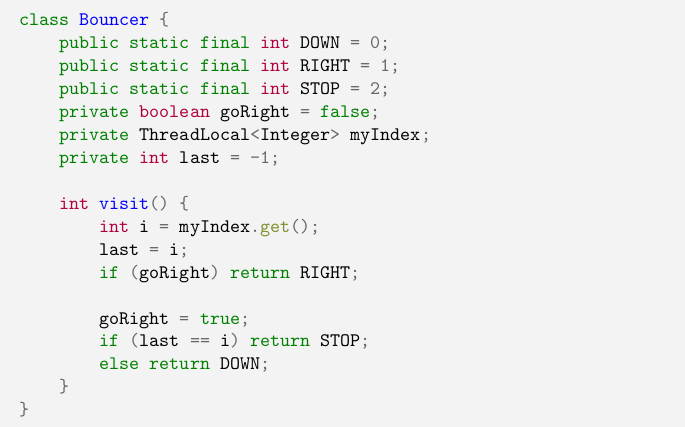
\includegraphics[width=0.7\textwidth]{final.png}\\
\end{center}

\begin{itemize}
\item[a) ]A lo m\'as un hilo obtiene el valor STOP
\item[b) ]A lo m\'as n - 1 hilos obtienen el valor DOWN
\item[c) ]A lo m\'as n - 1 obtienen el valor RIGHT
\end{itemize}

Respuesta:\\
Debemos mostrar qu\'e, como m\'aximo, un subproceso obtiene el valor STOP.
El punto clave es que el último puede ser el ID de, como máximo, uno de los hilos que
lee goRight + para que sea falso en la declaraci\'on if.
Podemos concluir esto porque sabemos: 
\begin{center}
$last.write(i) \rightarrow goRight.read(false) \rightarrow goRight.write(true) \rightarrow last.read(i) \rightarrow return(STOP)$
\end{center}

Para que dos hilos A y B hayan devuelto STOP, habrían tenido que leer sus identificadores en \'ultimo lugar. Sin p\'erdida de generalidad, digamos que B ley\'o por \'ultima vez despu\'es de que A ley\'o su valor allí.

\begin{center}
$A:last.read(A) \rightarrow B:last.read(B)$
\end{center}

Se deduce que B escribi\'o su valor en \'ultimo después de que A hab\'ia escrito y le\'ido su valor
all\'i (ya que A debe haber escrito su valor para haberlo le\'ido):

\begin{center}

$A:last.write(A) \rightarrow A:last.read(A) \rightarrow B:last.write(B) \rightarrow B:last.read(B)$
\end{center}

Pero de arriba sabemos qu\'e:

\begin{center}
$A:last.write(A) \rightarrow A:goRight.write(true) \rightarrow A:last.read(A)$
\end{center}
y

\begin{center}
$B:last.write(B) \rightarrow B:goRight.read(false) \rightarrow B : last.read(B)$
\end{center}

Uniendo hambas cosas tenemos qu\'e:


\begin{center}
$A:last.write(A) \rightarrow A:goRight.write(true) \rightarrow A:last.read(A) \rightarrow B:last.write(B) \rightarrow B:goRight.read(false) \rightarrow B:last.read(B)$
\end{center}

Dado que es imposible que cualquier hilo escriba false en goRight, no hay forma que el valor de goRight podr\'ia haberse vuelto falso una vez que A lo escribi\'o, contradiciendo B ley\'o de falso.
Por lo tanto, m\'as de un hilo no puede obtener el valor STOP. Aqu\'i están los pasos en la prueba.
\\ \\
Probar como m\'aximo los subprocesos $n-1$ obtienen el valor DOWN.

Para que cualquier hilo obtenga el valor DOWN, vemos que deben haber leído
GoRight para ser falso (para que no puedan regresar RIGHT). Asume n hilos
pudimos hacer esto. Luego de haber vuelto ABAJO, todos los hilos
han tenido que haber leído por última vez para ser desiguales a su valor. Pero como todo n
los subprocesos ya completaron la línea donde establecieron el último en su ID
no quedan otros hilos para cambiar el último valor. Sabemos que algunos
el subproceso debe haber sido el último en establecer el último en su ID, por lo que debe leer
esto y devolver STOP, contradiciendo nuestra suposición de que n hilos eran
capaz de regresar DOWN.



Probar que como máximo, los subprocesos n-1 obtienen el valor RIGHT.

En primer lugar, vemos las siguientes restricci\'ones para regresar a la DERECHA:


\begin{center}
$goRight.read(true) \rightarrow return(RIGHT)$
\end{center}

También notemos que goRight se inicializa en falso y que no hay escritura en goRight antes de que sea le\'ida por el primer hilo:

\begin{center}
$goRight.write(f alse) \rightarrow goRight.read(f alse) \rightarrow goRight.write(true)$
\end{center}
Entonces, el primer subproceso para verificar el valor de goRight debe encontrar que es falso,
haciendo que se salte la l\'inea para regresar a RIGHT. Por lo tanto, todos los n hilos no pueden
obtener el valor RIGHT ya que el primero no puede.


\end{itemize}




\end{document}